\documentclass[12pt]{article}
\usepackage[spanish,english,es-tabla]{babel}
\usepackage[utf8]{inputenc}
\usepackage[T1]{fontenc}
\usepackage{amssymb}
\usepackage{graphicx}
\usepackage{hyperref}
\begin{document}
	\selectlanguage{spanish}
	\title{Mini-taller de \LaTeX}
	\author{Raniita}
	\date{20 de marzo de 2020}
	\maketitle
	\pagebreak
	\section{Texto}
	\subsection{Fuentes}
	\subsubsection{Tipo}
	Hay muchas topografías distintas: \texttt{emph}, \texttt{textbf}, \texttt{texttt}, \texttt{underline}, \texttt{textnormal}\ldots
	\par
	\emph{enfática}
	\par 
	\textbf{negrita}
	\par 
	\texttt{máquina}
	\par
	\underline{subrayado} 
	\par
	\textnormal{normal}, \ldots
	\subsubsection{Tamaño}
	Hay gran cantidad de tamaños: \texttt{tiny}, \texttt{small}, \texttt{normalsize}, \texttt{Large}, \texttt{Huge}\ldots
	\par
	{\tiny minúsculo}
	\par 
	{\small pequeño}
	\par
	{\normalsize normal}
	\par 
	{\Large grande}
	\par 
	{\Huge enorme}, \ldots
	\subsection{Párrafos}
	\subsubsection{Espaciado}
	Éste es un párrafo. Punto y aparte. 
	\par
	Por defecto, el espacio entre párrafos es pequeño.
	\par\smallskip
	Pero se puede aumentar un poco (\texttt{smallskip}).
	\par\medskip
	Un poco más (\texttt{medskip}).
	\par\bigskip
	Más todavía (\texttt{bigskip}).
	\par\vspace{2cm}
	Incluso hacer tan grande como quieras (\texttt{vspace}).
	\par\bigskip\noindent
	Y, si no te gusta, puedes eliminar la indentación (\texttt{noindent}).
	\subsubsection{Sílabas} 
	\LaTeX\ separa automáticamente las sílabas: 
	\par
	esternoclideomastoideo esternoclideomastoideo esternoclideomastoideo esternoclideomastoideo esternoclideomastoideo esternoclideomastoideo esternoclideomastoideo esternoclideomastoideo esternoclideomastoideo esternoclideomastoideo 
	\par\bigskip\noindent
	Se puede forzar el cambio de línea para evitar desbordamientos (\texttt{linebreak}):
	\par
	esternoclideomastoideo esternoclideomastoideo esternoclideomastoideo \linebreak esternoclideomastoideo esternoclideomastoideo esternoclideomastoideo esternoclideomastoideo esternoclideomastoideo esternoclideomastoideo esternoclideomastoideo 
	\par\bigskip\noindent
	La separación puede ser distinta en inglés: \selectlanguage{english}
	\par
	esternoclideomastoideo esternoclideomastoideo esternoclideomastoideo esternoclideomastoideo esternoclideomastoideo esternoclideomastoideo esternoclideomastoideo esternoclideomastoideo esternoclideomastoideo esternoclideomastoideo 
	\par\bigskip\noindent
	Se le puede enseñar a \LaTeX\ las sílabas:
	\par
	es\-ter\-no\-cli\-deo\-mas\-toi\-de\-o es\-ter\-no\-cli\-deo\-mas\-toi\-de\-o es\-ter\-no\-cli\-deo\-mas\-toi\-de\-o es\-ter\-no\-cli\-deo\-mas\-toi\-de\-o es\-ter\-no\-cli\-deo\-mas\-toi\-de\-o es\-ter\-no\-cli\-deo\-mas\-toi\-de\-o es\-ter\-no\-cli\-deo\-mas\-toi\-de\-o es\-ter\-no\-cli\-deo\-mas\-toi\-de\-o es\-ter\-no\-cli\-deo\-mas\-toi\-de\-o es\-ter\-no\-cli\-deo\-mas\-toi\-de\-o 
	\selectlanguage{spanish}
	\par\bigskip\noindent
	También se pueden hacer párrafos alineados a izquierda o derecha sin separar en sílabas con los entornos \texttt{flushleft} y \texttt{flushright}:
	\begin{flushleft}
		esternoclideomastoideo esternoclideomastoideo esternoclideomastoideo esternoclideomastoideo esternoclideomastoideo esternoclideomastoideo esternoclideomastoideo esternoclideomastoideo esternoclideomastoideo esternoclideomastoideo 
	\end{flushleft}
	\begin{flushright}
		esternoclideomastoideo esternoclideomastoideo esternoclideomastoideo esternoclideomastoideo esternoclideomastoideo esternoclideomastoideo esternoclideomastoideo esternoclideomastoideo esternoclideomastoideo esternoclideomastoideo 
	\end{flushright}
	Y, por supuesto, centrados (\texttt{center}):
	\begin{center}
		esternoclideomastoideo esternoclideomastoideo esternoclideomastoideo esternoclideomastoideo esternoclideomastoideo esternoclideomastoideo esternoclideomastoideo esternoclideomastoideo esternoclideomastoideo esternoclideomastoideo 
	\end{center}
	\subsection{Listas}
	\subsubsection{Sin etiqueta}
	Se pueden hacer con el entorno \texttt{itemize}:
	\begin{itemize}
		\item Lo mismo te digo una cosa 
		\item Que te digo la otra
	\end{itemize}
	Se pueden añadir etiquetas opcionales de forma manual entre \texttt{[ ]}:
	\begin{itemize}
		\item[L-V:] Estudiar
		\item[SD:] Salir de fiesta
	\end{itemize}
	\subsubsection{Enumeradas}
	El \texttt{enumerate} se baila así:
	\begin{enumerate}
		\item El brikidans
		\item El cruzaíto
		\item El maiquelyason
		\item El robocop
	\end{enumerate}
	Las listas (\texttt{itemize} o \texttt{enumerate}) se pueden encajar unas con otras:
	\begin{enumerate}
		\item ¿Dónde se baila?
		\begin{enumerate}
			\item En China
			\item Y también en Alcorcón
		\end{enumerate}
		\item ¿Quién lo baila?
		\begin{enumerate}
			\item Mariano
			\item José Luis
		\end{enumerate}
	\end{enumerate}
	Incluso se puede iniciar los contadores donde se quiera:
	\begin{enumerate}
		\setcounter{enumi}{1}
		\item ¿Quién lo baila? (continuación)
		\begin{enumerate}
			\setcounter{enumii}{2}
			\item Mi hermano
			\item Mi mulata
		\end{enumerate}
	\end{enumerate}
	\section{Fórmulas}
	\subsection{Ubicación}
	\subsubsection{Dentro del texto}
	Una fórmula puede aparecer dentro de un texto entre \texttt{\$ \$}: $e=m\cdot c^2$. 
	\par\bigskip\noindent
	A veces interesa recuadrarlas con \texttt{fbox}: \fbox{$e=m\cdot c^2$}
	\par\bigskip\noindent
	Observa el efecto de \texttt{displaystyle}: $c=\sqrt{\frac{e}{m}} \neq \sqrt{\displaystyle\frac{e}{m}}$. 
	\par\bigskip\noindent
	Las fracciones, los límites, las sumas, máximos o las integrales pueden representarse de formas distintas: $\lim_{n\to\infty}\sum_{m=1}^n\max_{n \in \mathbb{N}}\int_a^b$ no necesita un espacio vertical adicional, pero $\displaystyle\lim_{n\to\infty}\sum_{m=1}^n\max_{n \in \mathbb{N}}\int_a^b$ sí.
	\subsubsection{Externas}
	Normalmente, las fórmulas se ven mejor fuera del texto:
	\[
	c=\sqrt{\displaystyle\frac{e}{m}}
	\]
	Se pueden numerar con \texttt{equation} y usar las etiquetas (\texttt{label}, \texttt{ref})
	\begin{equation}\label{energia}
	e=m \cdot c^2
	\end{equation}
	\begin{equation}\label{masa}
	m=\displaystyle\frac{e}{c^2}
	\end{equation}
	(\ref{energia}) y (\ref{masa}) son ecuaciones equivalentes.
	\subsection{Índices}
	En \LaTeX\ existen tanto índices como superíndices: $a_{i,j}^k$. 
	\par\bigskip\noindent
	Pero cuidado al poner índice dobles: ${a^b}^c \neq a^{bc}$, ${a_i}_j \neq a_{ij}$
	\par\bigskip\noindent
	También se pueden poner en sumas, integrales, límites, máximos, \ldots
	\[
	\sum_{n=0}^{\infty} \ \lim_{n \to \infty} \max_{x \in \mathbb{R}} \int_{x=a}^{x=b}
	\]
	\subsection{Letras griegas}
	Las minúsculas son muy sencillas:
	\[
	\alpha \ \beta \ \gamma \ \delta \ \epsilon \ldots 
	\]
	Algunas de las mayúsculas coinciden con nuestro alfabeto:
	\[
	A \ B \ \Gamma \ \Delta \ E \ldots 
	\]
	Algunas letras admiten dos expresiones:
	\[
	\epsilon \neq \varepsilon , \ \phi \neq \varphi, \ \theta \neq \vartheta \ldots 
	\]
	\subsection{Texto en fórmulas}
	\subsubsection{Tipografía}
	Hay que diferenciar el texto de las fórmulas:
	\[
	texto matem\acute{a}tico \neq \textnormal{texto normal}
	\]
	Aunque es inusual usar acentos en matemáticas, hay otro tipo de símbolos similares: barras, flechas, tildes
	\[
	\acute{a} \ \hat{a} \ \vec{a} \ \bar{a} \ \tilde{a} \ \dot{a}
	\]
	\subsubsection{Espaciado}
	Hay múltiples opciones de espaciado en una fórmula:
	\[
	a b \, c \ d \hspace{1cm} e
	\]
	Se puede utilizar espaciado negativo:
	\[
	a\!b \ a\hspace{-2pt}b 
	\]
	\subsection{Apertura y clausura}
	Puede que necesitemos paréntesis grandes que se ajusten a una fórmula (\texttt{left}, \texttt{right}):
	\[
	(\sqrt{2}^{\sqrt{2}})^{\sqrt{2}} \neq \left(\sqrt{2}^{\sqrt{2}}\right)^{\sqrt{2}}
	\]
	Ademś de paréntesis, podríamos necesitar corchetes, llaves\ldots Es posible encontrase solo con apertura o clausura (\texttt{left.} o \texttt{right.}):
	\[
	\int_a^b x^n\,dx=\left.\frac{x^{n+1}}{n+1}\right|_a^b=\frac{b^{n+1}-a^{n+1}}{n+1}
	\]
	\subsection{Fórmulas con varias líneas}
	\subsubsection{Alineación}
	Un ejemplo de \texttt{array} pueden ser funciones definidas a trozos:
	\[
	|x|=
	\left\{
	\begin{array}{cl} 
	x  & \textnormal{si }x \geq 0 \\
	-x & \textnormal{si }x \leq 0
	\end{array}
	\right.
	\]
	Se suelen alinear los signos de igualdad (\texttt{r}ight, \texttt{c}enter, \texttt{l}eft):
	\[
	\begin{array}{rcll}
	(a+b)^2&=&a^2+2ab+b^2 & \textnormal{si }a,b\in\mathbb{R} \\ 
	(A+B)^2&=&A^2+A \cdot B+B \cdot A+B^2 & \textnormal{si }A,B\in\mathcal{M}_n(\mathbb{R})
	\end{array}
	\]
	\subsubsection{Matrices}
	Las matrices son un caso particular de fórmula de varias líneas:
	\[
	\left(
	\begin{array}{c}
	n \\
	m
	\end{array}
	\right)=\frac{n!}{m! \cdot (n-m)!} \textnormal{ si }n \geq m \geq 0
	\]
	A veces es necesario utilizar espacios verticales extra \texttt{[ ]}, o puntos suspensivos direccionales (\texttt{ldots}, \texttt{cdots}, \texttt{vdots}, \texttt{ddots}):
	\[
	A=\left(
	\begin{array}{c}
	\displaystyle\int_a^b x \, dx \\
	\displaystyle\sum_{n=0}^\infty a_n 
	\end{array}
	\right) 
	\qquad
	B=\left(
	\begin{array}{c}
	\displaystyle\int_a^b x \, dx \\ [0.5cm]
	\displaystyle\sum_{n=0}^\infty a_n 
	\end{array}
	\right)
	\qquad
	C=
	\left(
	\begin{array}{ccc}
	a_{1\,1} & \ldots & a_{1\,n} \\
	\vdots   & \ddots & \vdots \\
	a_{m\,1} & \ldots & a_{m\,n}
	\end{array}
	\right)
	\]
	\section{Objetos flotantes}
	\subsection{Tablas}
	Las tablas no se diferencian mucho de los \texttt{array} del modo matemático, aunque se pueden incluir en un entorno \texttt{table} específico:
	\begin{table}[t]
		\begin{center}
			\begin{tabular}{|c|c|}\hline
				Dorsal & Nombre \\ \hline \hline
				1      & Ter Stegen   \\ \hline
				3      & Gerard Piqué \\ \hline
				4      & Ivan Rakitić \\ \hline
				\vdots & \vdots       \\ \hline
			\end{tabular}
		\end{center}
		\caption{Plantilla del F.C.~Barcelona arriba}
	\end{table}
	\begin{table}[h]
		\begin{center}
			\begin{tabular}{|c|c|}\hline
				Dorsal & Nombre \\ \hline \hline
				1      & Ter Stegen   \\ \hline
				3      & Gerard Piqué \\ \hline
				4      & Ivan Rakitić \\ \hline
				\vdots & \vdots       \\ \hline
			\end{tabular}
		\end{center}
		\caption{Plantilla del F.C.~Barcelona aquí}
	\end{table}
	\begin{table}[b]
		\begin{center}
			\begin{tabular}{|c|c|}\hline
				Dorsal & Nombre \\ \hline \hline
				1      & Ter Stegen   \\ \hline
				3      & Gerard Piqué \\ \hline
				4      & Ivan Rakitić \\ \hline
				\vdots & \vdots       \\ \hline
			\end{tabular}
		\end{center}
		\caption{Plantilla del F.C.~Barcelona abajo}
	\end{table}
	Nótese que cada tabla aparece en una posición (flotante) diferente: \texttt{t}op, \texttt{h}ere, \texttt{b}ottom.
	\subsection{Gráficas}
	No es imprescindible, pero se suele usar un entorno \texttt{figure} similar al \texttt{table}. Se pueden ajustar ancho o alto (\texttt{width}, \texttt{heigth}), y crear dos (o más) gráficas al mismo nivel creando minipáginas (\texttt{minipage}):
	\begin{figure}[h]
		\begin{center}
			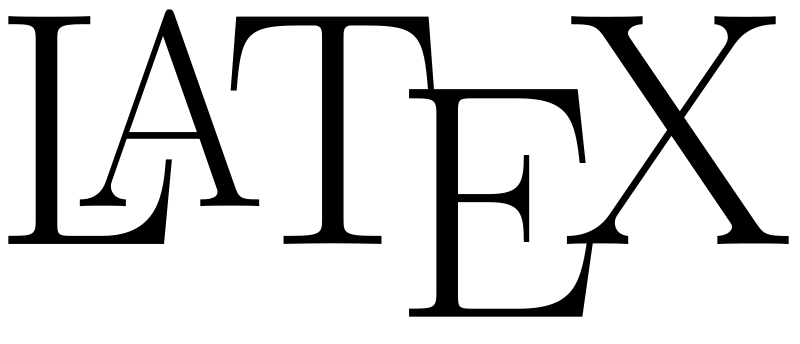
\includegraphics{latex_logo.png}
			\caption{Sin tener en cuenta el tamaño (enorme desbordamiento)}
		\end{center}
	\end{figure}
	\begin{figure}[h]
		\begin{center}
			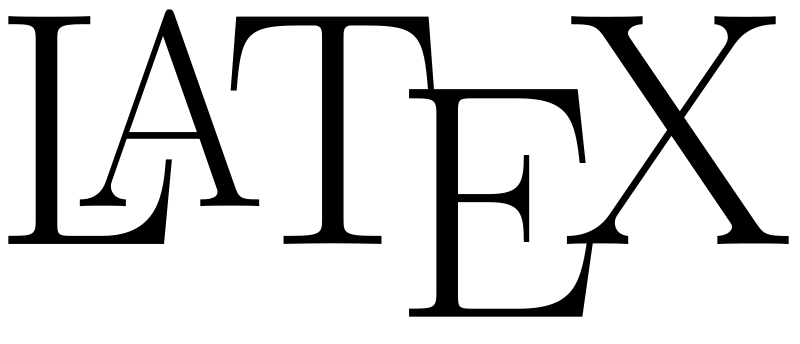
\includegraphics[width=0.8\textwidth]{latex_logo.png}
			\caption{Ajustando al ancho}
		\end{center}
	\end{figure}
	\begin{figure}[h]
		\begin{minipage}{0.5\linewidth}
			\begin{center}
				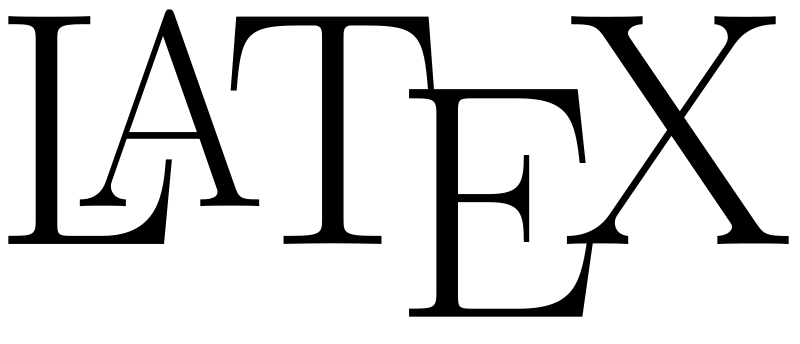
\includegraphics[width=0.4\textwidth]{latex_logo.png}
			\end{center}
		\end{minipage}
		\begin{minipage}{0.5\linewidth}
			\begin{center}
				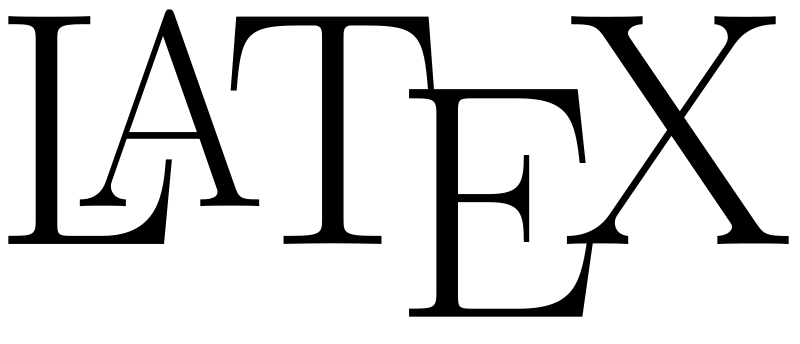
\includegraphics[width=0.4\textwidth]{latex_logo.png}
			\end{center}
		\end{minipage}
		\caption{Un único pie de figura para ambas gráficas}
		\vspace{1cm}
		\begin{minipage}{0.5\linewidth}
			\begin{center}
				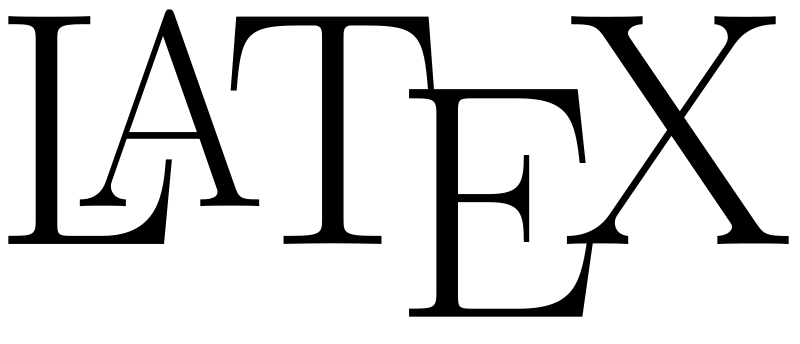
\includegraphics[width=0.4\textwidth]{latex_logo.png}
				\caption{Pie de figura izquierdo}
			\end{center}
		\end{minipage}
		\begin{minipage}{0.5\linewidth}
			\begin{center}
				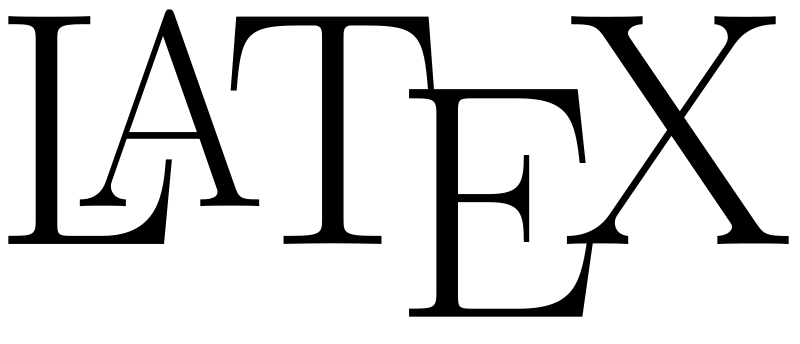
\includegraphics[width=0.4\textwidth]{latex_logo.png}
				\caption{Pie de figura derecho}
			\end{center}
		\end{minipage}
	\end{figure}
	\section{Referencias}
	\subsection{Enlaces}
	Con \texttt{href} se puede enlazar una \href{http://www.upct.es/}{Página web} o \href{file:latex_logo.png}{un archivo}
	\subsection{Índices}
	Se puede crear un índice de contenidos \texttt{tableofcontents}, tablas \texttt{listoftables} o figuras \texttt{listoffigures} en cualquier parte, aunque solo tiene sentido al principio (preferible) o al final:
	\tableofcontents
	\listoftables
	\listoffigures
	\subsection{Bibliografía}
	La bibliografía, como los libros \cite{libro} y \cite[cap.~3]{otro_libro}, o el artículo \cite[pág.~12]{articulo}, se suele incluir en un apartado al final.
	\begin{thebibliography}{9}
		\bibitem{libro} Un libro
		\bibitem{otro_libro} Otro libro
		\bibitem{articulo} Un artículo
	\end{thebibliography}
\end{document}